\chapter{MQTT Binding}
\begin{figure}
    \centering
    
\includegraphics{Immagini/mqtt_logo.png}
    \caption{MQTT Logo}
    \label{fig:mqtt_logo}
\end{figure}

Come già spiegato alla sezione \ref{chap:binding_intro} un {\em binding} permette di connettere un dispositivo fisico ad una {\em thing}. In questo caso specifico \'e stato sviluppato un {\em sistema IOT} per sperimentare l'associazione con openHAB. Per collegare il device ed il framework \'e stato utilizzato il protocollo di rete \textbf{MQTT}.

\section{Protocollo MQTT}
{\em Message Queuing Telemetry Transport} \'e un protocollo di rete leggero di tipo {\em  publish-subscribe} che funziona su TCP/IP. MQTT \'e progettato per connessioni con postazioni remote in cui è richiesta un'impronta di codice ridotta o una larghezza di banda della rete limitata \cite{enwiki:1023769301}.

Il protocollo definisce due tipi di entit\'a di rete:
\begin{itemize}
    \item \textbf{broker}
    \item \textbf{client}
\end{itemize}
Esse vengono illustrate a Figura \ref{fig:mqtt_model_structure}.

\begin{figure}
    \centering
    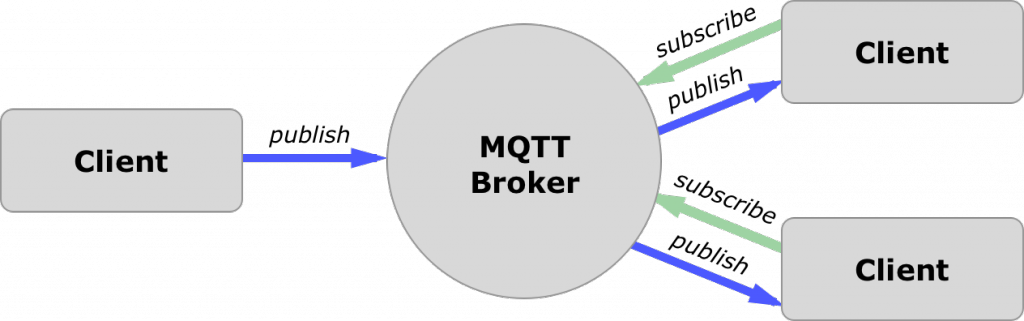
\includegraphics[width=12cm]{Immagini/mqtt_model_structure.png}
    \caption{MQTT Model Structure}
    \label{fig:mqtt_model_structure}
\end{figure}

\paragraph{broker} server che riceve tutti i messaggi dai {\em client} e li instrada ai {\em client} di destinazione appropriati. Il {\em broker MQTT} \'e un software in esecuzione su un computer in locale o remoto. Di esso sono disponibili sia implementazioni open source che proprietarie. Il {\em broker} riceve solitamente messaggi da un {\em publisher} che distribuisce a pi\'u {\em subscriber}. Sia il {\em publisher} che il {\em subscriber} sono {\em client MQTT}. Il {\em broker} mantiene traccia di tutte le informazioni della sessione mentre i dispositivi si accendono e si spengono. Esse vengono chiamate {\em persistent sessions}.

\paragraph{client} qualsiasi dispositivo che esegue una libreria MQTT per connettersi ad un broker MQTT in rete. Un {\em client} ha dialogo diretto solamente con un broker e non con altri {\em client}; il broker infatti fa da tramite tra lui e gli altri. I {\em client} possono {\em pubblicare} o {\em sottoscriversi} per inviare o riceve dati.

\paragraph{topic} le informazioni sono organizzate in gerarchie di argomenti chiamati {\em topic}. Quando un {\em client} vuole inviare un messaggio ad un altro, basta che lo invia al broker con lo stesso {\em topic} a cui \'e sottoscritto il {\em client}. 

\paragraph{retained message} Se viene inviato un messaggio al {\em broker} relativo ad un {\em topic} dove non vi sono {\em client} sottoscritti viene scartato. Ci\'o non viene fatto nel caso di {\em retained message}. Esso \'e un normale messaggio MQTT con flag {\em retain} a true. In caso viene inviato un {\em retained message}, questo viene memorizzato insieme al rispettivo QoS. In tal caso quindi possono essere salvati gli ultimi messaggi nei propri {\em topic} cos\'i da notificare un subscriber degli ultimi dati inviati appena si sottoscrive.

\paragraph{message types} sono utizzati durante la connessione illustrata a Figura \ref{fig:mqtt_connection}.
\begin{itemize}
    \item \textbf{connect}: aspetta una connessione con il {\em broker} e crea un collegamento tra i nodi
    \item \textbf{disconnect}: attende la terminazione del lavoro da parte del {\em client} e la disconnessione della sessione TCP/IP.
    \item \textbf{publish}: ritorna il messaggio inviato da un {\em client MQTT} al broker immediatamente al thread dell'applicazione di ogni client sottoscritto allo stesso topic.
\end{itemize}

\begin{figure}
    \centering
    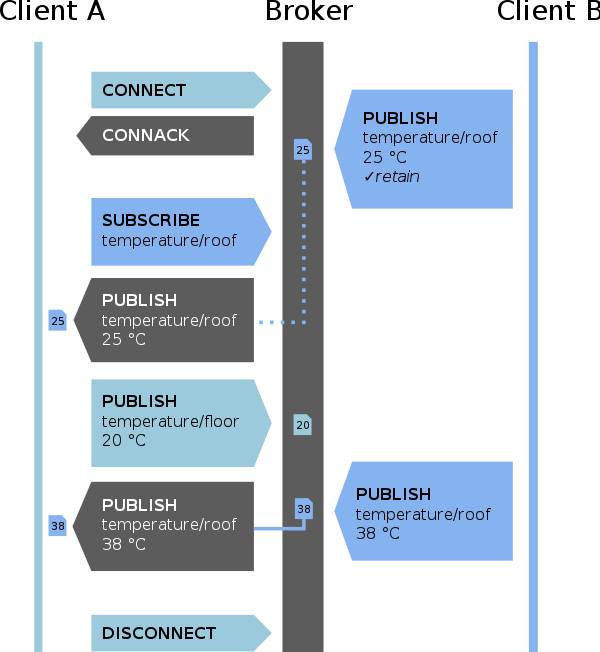
\includegraphics[width=12cm]{Immagini/mqtt_connection.png}
    \caption{MQTT Connection}
    \label{fig:mqtt_connection}
\end{figure}

\section{openHAB Binding}
{\em openHAB} implementa un {\em binding} gi\'a configurato per il protocollo MQTT. Tale protocollo ha un'architettura client/server. Il server di MQTT, ovvero il {\em broker} NON viene fornito nel binding di openHAB ma pu\'o essere utilizzato qualsiasi altro software che f\'a da {\em broker MQTT} come {\em Mosquitto}. Il {\em binding openHAB} permette di configurare le connessioni ai broker tramite le {\em openHAB things}. L'associazione non permette per\'o di collegare i {\em channels} ai {\em topic} o di eseguire il rilevamento automaticodei {\em topic} disponibili. I {\em bridge} supportati sono: 

\begin{itemize}
    \item \textbf{Broker}: {\em bridge} che rappresenta una connessione {\em broker MQTT} configurata e gestita da tale {\em binding}.
    \item \textbf{SystemBroker}: un {\em broker} configurato dal sistema non pu\'o essere modificato da questo {\em binding} e verr\'a elencato come {\em broker} di sistema di sola lettura.
\end{itemize}

\subsection{Configurazione bridge}
\begin{itemize}
    \item \textbf{host}: IP/hostname del broker MQTT. {\em Binding} che consente una connessione univoca con {\em host:porta}.
    \item \textbf{port}: se non ne viene fornita nessuna vengono utilizzate quelle di default che sono 1883 e 8883(SSL). {\em Binding} che consente una connessione univoca con {\em host:porta}.
    \item \textbf{secure}: se si vuole utilizzare una connessione sicura con il {\em broker} tramite TLS/SSL. Pu\'o essere true o false. Di default \'e false.
\end{itemize}

Altri parametri da impostare possono essere:
\begin{itemize}
    \item \textbf{qos}: indica qualit\'a del servizio che pu\'o essere imposrtata a 0, 1 o 2 (default 0).
    \item \textbf{clientID}: ID client fisso che viene generato automaticamente.
\end{itemize}

I parametri di riconnessione sono:
\begin{itemize}
    \item \textbf{reconnectTime}: tempo di riconnessione in millisecondi. Valore del tempo di attesa aspettato per una connessione dopo che ne viene persa una. Il valore predefinito \'e 60000 (60s).
    \item \textbf{keepAlive}: tempo in secondi utile per capire se una connessione al server \'e persa o no. IL valore di default \' 60s.
\end{itemize}

Pu\'o essere impostato un LWT(testamento) MQTT:
\begin{itemize}
    \item \textbf{lwtMessage}: messaggio del testamento. Default vuoto.
    \item \textbf{lwtTopic}: topic del testamento. Default vuoto.
    \item \textbf{lwt}: qos del testamento. Default 0.
    \item \textbf{lwtRetain}: conserva l'ultimo messaggio. True o false, false di default.
\end{itemize}

Inoltre si possono impostare i seguenti parametri opzionali:
\begin{itemize}
    \item \textbf{username}: nome utente MQTT
    \item \textbf{password}: password MQTT
    \item \textbf{certificatepin}: se impostato dopo che \'e stata stabilita una connessione controlla il certificato. Se questo risulta non essere valido viene interrotta la connessione. Questa opzione aumenta la sicurezza.
    \item \textbf{publickeypin}: se impostata dopo che \'e stata stabilita una connessione controlla la chiave pubblica. Se questa risulta non essere valida viene interrotta la connessione. Questa opzione aumenta la sicurezza.
    \item \textbf{certificate}: hash del certificato utile per verificarne l'autenticit\'a per mezzo di {\em certificatepin}.
    \item \textbf{publickey}: hash della chiave pubblica utile per verificarne l'autenticit\'a per mezzo di {\em publickeypin}.
    \item \textbf{enableDiscovery}: di default sono abilitati i servizi di rilevamento sul broker. Questi possono essere controllati per mezzo di tale parametro.
\end{itemize}

\subsection{Things supportate}
Data la struttura molto generica di MQTT, il {\em binding}  consente di aggiungere un numero arbitrario di {\em thinngs MQTT} generiche. Su ogni {\em thing} possono essere aggiunti un numero arbitrario di {\em channels}.

\subsubsection{Channels supportati}
\begin{itemize}
    \item \textbf{string}: invia o riceve del testo su un {\em topic MQTT}.
    \item \textbf{number}: invia o riceve un numero su un {\em topic MQTT}.
    \item \textbf{dimmer}: gestisce un valore percentuale.
    \item \textbf{contact}: rappresenta uno stato di OPEN/CLOSE.
    \item \textbf{switch}: invia o riceve uno stato ON/OFF su un {\em topic MQTT}.
    \item \textbf{color}: gestisce i valori di un colore nei formati HSB, RGB o xyY (x, y, luminosit\'a)..
    \item \textbf{location}: gestisce una posizione.
    \item \textbf{image}: gestisce un'immagine binaria nei formati supportati da Java (bmp, jpg, png).
    \item \textbf{datetime}: gestisce un valore data/ora.
    \item \textbf{rollershutter}: gestisce una tapparella.
\end{itemize}

\subsection{Configurazione channel}
\begin{itemize}
    \item \textbf{stateTopic}: {\em topic MQTT} che rappresenta lo stato della {\em thing}. Possono essere utilizzati caratteri jolly per recuperare lo stato da pi\'u {\em topic}.
    \item \textbf{trasformationPattern}: pattern di trasformazione opzionale applicato a tutti i valori di entrata.
    \item \textbf{trasformationPatternOut}: pattern di trasformazione opzionale applicato a tutti i valori di uscita.
    \item \textbf{commandTopic}: {\em topic} per inviare comandi in uscita. Se non viene impostato il {\em channel} \'e in modalit\'a read-only.
    \item \textbf{formatBeforPublish}: utile per formattare un valore prima che viene pubblicato nel {\em broker MQTT}. Di default \'e utilizzato per il passaggio tra {\em channel} e {\em item}.
    \item \textbf{postCommand}: azione che permette di inviare ad altri elementi il valore ricevuto per un particolare {\em topic MQTT}.
    \item \textbf{retained}: verr\'a inviato il valore come messaggio MQTT mantenuto.
    \item \textbf{qos}: qos del {\em channel}.
    \item \textbf{trigger}: se true il {\em topic} dello stato aggiorner\'a un {\em channel} al suo posto.
\end{itemize}

\subsubsection{string}
\begin{itemize}
    \item \textbf{allowStates}: elenco separato da virgole di stati consentiti.
\end{itemize}


\subsubsection{number}
\begin{itemize}
    \item \textbf{min}: valore minimo
    \item \textbf{max}: valore massimo
    \item \textbf{step}: per canali aumenta o decrementa
    \item \textbf{unit}: unit\'a di misura
\end{itemize}

\subsubsection{contact, switch}
\begin{itemize}
    \item \textbf{on}: un numero opzionale (come 1, 10) o una stringa (come ``ON''/``Open'') riconosciuti come stato on/open.
    \item \textbf{off}: un numero opzionale (come 0, -10) o una stringa (come ``OFF''/``Close'') riconosciuti come stato off/close.
\end{itemize}

\subsubsection{color}
\begin{itemize}
    \item \textbf{color\_mode}: stringa obbligatoria che defisnisce la rappresentazione del colore: ``hsb'', ``rgb'', ``xyY''.
    \item \textbf{on}: una stringa facoltativa (come ``BRIGHT'') riconoscita come on.
    \item \textbf{off}: una stringa facoltativa (come ``DARK'') riconoscita come off.
    \item \textbf{onBrightness}: se collegato ad un {\em item} switch ed \'e acceso.
\end{itemize}

\subsubsection{location}
Pu\'o essere collegato tale {\em channel} ad un {\em Location item}. Esso pubblicher\'a la posizione come elenco separato da virgole sul broker MQTT (esempio: ``112,54,123'', ovvero latitudine, longitudine e altitudine).

\subsubsection{image}
Pu\'o essere collegato tale {\em channel} ad un {\em Image item} ed \'e di tipo read-only. I valori devono essere in binario e del formato supportato da java (bmp, jpg, png).

\subsubsection{datetime}
Pu\'o essere collegato tale {\em channel} ad un {\em DateTime item}. Pubblicher\'a la data/ora nel formato ``aaaa-MM-gg'T'HH::mm''.

\subsubsection{rollershutter}
\begin{itemize}
    \item \textbf{on}: stringa facoltativa come ``Open'' riconosciuta come UP.
    \item \textbf{off}: stringa facoltativa come ``Close'' riconosciuta come DOWN.
    \item \textbf{stop}: stringa facoltativa come ``Stop'' riconosciuta come STOP.
\end{itemize}

\subsection{Rule actions}
Tale {\em binding} include una regola di azione che consente di pubblicare messaggi MQTT dall\'interno. delle regole.

\begin{lstlisting}[caption=Esempio Rule Action Istanza,label=code:rule_action_example_instance]
val mqttActions = getActions("mqtt","mqtt:systemBroker:embedded-mqtt-broker")
\end{lstlisting}

Nel Codice \ref{code:rule_action_example_instance} il primo parametro deve essere sempre \texttt{mqtt} mentre il secondo \'e il Thing UID del broker usato. Una volta recuparata l'stanza d'azione basta pubblicare con in comando \texttt{publishMQTT(String topic, String value, Boolean retain)} come nel Codice \ref{code:rule_action_example_publish}.

\begin{lstlisting}[caption=Esempio Rule Action Pubblicazione,label=code:rule_action_example_publish]
mqttActions.publishMQTT("mytopic","myvalue", true)
\end{lstlisting}